
\section{Die W-/Z-Boson Entdeckung}

\chapterauthor{Jean-Marco Alameddine, 07.12.2018}

\subsection{Historische Entwicklung der schwachen Wechselwirkung}

Die Geschichte der theoretischen Beschreibung der schwachen Wechselwirkung geht zurück auf Fermi im Jahre 1933.
Er beschrieb den $\beta^-$-Zerfall über eine direkte Vier-Fermionen Wechselwirkung ohne Austauschteilchen.
Während diese Theorie für kleine Energien (verglichen mit der Masse der heute bekannten Eichbosonen W und Z) eine gute Näherung beschreibt, treten für höhere Energien theoretische Probleme und experimentelle Diskrepanzen in Fermis Theorie auf.
Trotzdem stellte diese Theorie der schwachen Wechselwirkung über viele Jahre hinweg eine gute Vorhersage dar, die auf viele Prozesse angewendet sowie an neue Phänomene wie die Paritätsverletzung angepasst werden konnte.

Um Probleme wie die Divergenzen in höheren Ordnungen bzw. bei hohen Energien zu beheben beschrieben Glashow, Weinberg und Salam im Jahre 1968 die elektroschwache Wechselwirkung.
Es handelt sich dabei um eine vereinheitlichte Theorie der Quantenelektrodynamik und der schwachen Wechselwirkung.
Vorhersagen die durch diese Theorie getroffen werden sind insbesondere das masselose Photon sowie die massebehafteten Austauschteilchen $\text{W}^+$, $\text{W}^-$ und $\text{Z}^0$.
Aufgrund von Letzterem werden innerhalb der elektroschwachen Theorie sogenannte neutrale Ströme vorhergesagt, bei denen ein Neutrino mit einem leptonischen oder hadronischen Teilchen unter Austausch eines $\text{Z}^0$-Bosons wechselwirkt.

Dieses Phänomen konnte im Juli 1973 mithilfe des Gargamelle Detektors, einer Blasenkammer am CERN, nachgewiesen werden.
Hierbei wird ein fokussierter Neutrinostrahl auf eine mit Freon gefüllte Kammer gelenkt. 
Mithilfe von Lichtblitzen und Kameras werden ionisierende Teilchen, die Gasblasen als Spur hinterlassen, nachgewiesen.
Hierbei konnte die eindeutige Signatur von neutralen Strömen nachgewiesen werden, welche durch die elektroschwache Theorie vorhergesagt wurden.
Zudem konnten die Massen der in dieser Theorie enthaltenen Bosonen zu 
\begin{align*}
	M_\text{W} &\approx \left(60-80\right)\si{\giga\electronvolt}\\
	M_\text{Z} &\approx \left(75-92\right)\si{\giga\electronvolt}
\end{align*}
abgeschätzt werden.
Zum Zeitpunkt der Entdeckung existiere jedoch kein Experiment mit ausreichender Schwerpunktsenergie $\sqrt{s}$ um diese Teilchen tatsächlich zu erzeugen und somit eindeutig nachzuweisen.

\subsection{Beschleuniger zur Entdeckung der W- und Z-Bosonen}
Seit Juni 1976 war am CERN das Super Proton Synchrotron (SPS) im Betrieb.
Es handelte sich dabei um ein Fixed-Target Experiment für Protonen, wobei diese auf eine Strahlenergie von $E = \SI{400}{\giga\electronvolt}$ beschleunigt wurden.
Als Schwerpunktsenergie steht hierbei jedoch nur eine Energie von $\sqrt{s} = \sqrt{2 E m} \approx \SI{27}{\giga\electronvolt}$ zur Verfügung, was nicht zum Nachweis des W- oder Z-Bosons ausreicht.

Eine mögliche Idee, um höhere Schwerpunktsenergien zu erreichen, stellen Collding-Beam-Experimente dar.
Für Proton-Proton Kollisionen beträgt die Schwerpunktsenergie, unter Berücksichtigung der Partonstruktur der Hadronen, $\sqrt{s} = 2 \cdot E \cdot x$ mit $x \approx \num{0.2}$.
Eine Weiterentwicklung dieser Idee von Carlo Rubbia und Peter McIntyre war es, anstatt Proton-Proton Kollisionen, Protonen mit Antiprotonen kollidieren zu lassen.
Hierzu wäre es ausreichend, ein bestehendes Proton-Synchrotron umzubauen, so dass Protonen und Antiprotonen entgegengesetzt in derselben Vakuumröhre beschleunigt werden können.
Auf Grundlage dieser Idee wurde im Januar 1978 begonnen, das SPS in einen Proton-Antiproton-Collider, das Super Proton Antiproton Synchrotron (Sp$\overline{\text{p}}$S) umzubauen.
Hierbei konnten bei einer Strahlenergie von $E = \SI{300}{\giga\electronvolt}$ Schwerpunktsenergien von etwa $\sqrt{s} = \SI{120}{\giga\electronvolt}$ erreicht werden, was für die vorhergesagte Erzeugung der massebehafteten Eichbosonen der schwachen Wechselwirkung ausreichend ist.

Das Sp$\overline{\text{p}}$S wurde von Juli 1981 bis 1991 als Speicherring für Protonen und Antiprotonen betrieben.
Hierzu war es insbesondere nötig, das Vakuum in der Röhre deutlich zu verbessern sowie die entgegengesetzte Injektion und Beschleunigung in dieser Röhre zu ermöglichen.
Um eine ausreichende Anzahl von Antiprotonen für den Speicherring zu erzeugen wurde der Antiproton Accumulator (AA) verwendet.
Die Antiprotonen werden erzeugt, indem ein Protonenstrahl vom Proton Synchrotron (PS) auf ein Target geleitet wird.
Die entstehenden Antiprotonen werden mit einem Spektrometer ausgewählt und in den AA geleitet.
Um die Antiprotonen für das Sp$\overline{\text{p}}$S verwenden zu können muss insbesondere der Phasenraum der Antiprotonen verkleinert werden.
Hierzu wird das Prinzip der stochastischen Kühlung verwendet, welches von Simon van der Meer 1972 entwickelt wurde:
Teilchen bzw. Teilchengruppen, welche nicht der Idealbahn im Speicherring folgen, führen Oszillationen durch.
Um diese zu unterdrücken werden die Abweichungen mithilfe eines "Pick-up" gemessen und ein Signal ausgegeben.
Dieses wird vom einem "Kicker" aufgenommen und eine elektromagnetische Korrektur auf den Teilchenstrahl angewendet.
Hierdurch konnte der Phasenraum um einen Faktor $\num{1e9}$ reduziert werden.

\subsection{Detektoren zur Entdeckung der W- und Z-Bosonen}

Zum Nachweis der Signaturen der W- und Z-Bosonen wurden zwei Experimente am Sp$\overline{\text{p}}$S errichtet:
Das Experiment UA1 war ein großer, multifunktionaler $4\pi$-Detektor mit Driftkammer, Kalorimetern und Myonkammern.
Im Gegensatz dazu war das zweite Experiment, UA2, spezialisiert auf den Nachweis von Elektronen unter Nutzung von präzisen, hochaufgelösten Kalorimetern.

Das nachzuweisende W-Boson zerfällt primär in ein Quark-Antiquark-Paar, welches zwei Jets bildet.
Da diese Signatur jedoch stark überlagert ist durch Untergrund aus harter Streuung der Partonen wird das W-Boson durch die Signatur $\text{W} \rightarrow l \nu_l$ nachgewiesen.
Hierbei tritt ein isoliertes Elektron mit hohem transversalen Impuls auf sowie ein Neutrino, welches über einen fehlenden transversalen Impuls nachgewiesen werden kann.
Die von UA1 beobachteten Events mit einem Elektron mit hohem transversalen Impuls weisen, wie in Abbildung \ref{fig:boson} dargestellt, in allen Fällen einen antiparallel dazu liegenden fehlenden transversalen Impuls auf, der dem Neutrino zugeordnet werden kann.
Hierdurch konnte im Januar 1983 die Entdeckung des W-Bosons bekannt gegeben werden.

\begin{figure}
  \centering
  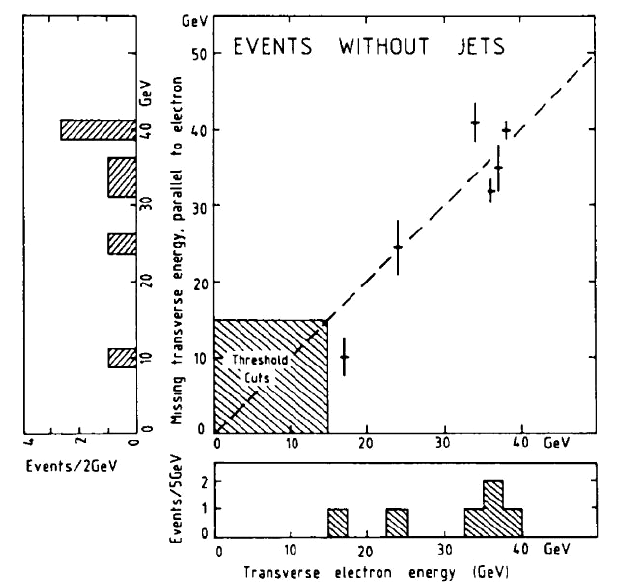
\includegraphics[height=10.0cm]{ressources/Screenshot_2018-12-04_18-22-25.png}
  \caption{Ergebnisse von UA1 aus dem Jahre 1982 \cite{boson}}
  \label{fig:boson}
\end{figure}

Die nachzuweisende Reaktion des W-Bosons ist $\text{Z} \rightarrow \text{e}^+ \text{e}^-$.
Als Signatur existieren dabei zwei Kalorimetereinträge, auf die jeweils eine isolierte Spur eines Elektrons zeigt.
An UA1 konnten vier solcher Ereignisse sowie ein Myon-Antimyon-Paar nachgewiesen werden, welche mit einer invarianten Masse von ca. $M_\text{Z} \approx \SI{95.2}{\giga\electronvolt}$ kompatibel sind.
Zusammen mit drei von UA2 gemessenen Ereignissen konnte im Juni 1983 die Entdeckung des Z-Bosons bekannt gegeben werden.

\subsection{Weitere Entwicklungen}

Für ihren Beitrag zur Entdeckung der W- und Z-Bosonen erhielten Carlo Rubbia und Simon van der Meer 1984 den Nobelpreis in Physik.

In den folgenden Jahrzehnten folgten Präzisionsmessungen der Massen $M_\text{Z}$ und $M_\text{W}$, die insbesondere am Tevatron sowie am Large-Electron-Positron Collider durchgeführt wurden.